\documentclass{article}\usepackage[]{graphicx}\usepackage[]{color}
%% maxwidth is the original width if it is less than linewidth
%% otherwise use linewidth (to make sure the graphics do not exceed the margin)
\makeatletter
\def\maxwidth{ %
  \ifdim\Gin@nat@width>\linewidth
    \linewidth
  \else
    \Gin@nat@width
  \fi
}
\makeatother

\definecolor{fgcolor}{rgb}{0.345, 0.345, 0.345}
\newcommand{\hlnum}[1]{\textcolor[rgb]{0.686,0.059,0.569}{#1}}%
\newcommand{\hlstr}[1]{\textcolor[rgb]{0.192,0.494,0.8}{#1}}%
\newcommand{\hlcom}[1]{\textcolor[rgb]{0.678,0.584,0.686}{\textit{#1}}}%
\newcommand{\hlopt}[1]{\textcolor[rgb]{0,0,0}{#1}}%
\newcommand{\hlstd}[1]{\textcolor[rgb]{0.345,0.345,0.345}{#1}}%
\newcommand{\hlkwa}[1]{\textcolor[rgb]{0.161,0.373,0.58}{\textbf{#1}}}%
\newcommand{\hlkwb}[1]{\textcolor[rgb]{0.69,0.353,0.396}{#1}}%
\newcommand{\hlkwc}[1]{\textcolor[rgb]{0.333,0.667,0.333}{#1}}%
\newcommand{\hlkwd}[1]{\textcolor[rgb]{0.737,0.353,0.396}{\textbf{#1}}}%

\usepackage{framed}
\makeatletter
\newenvironment{kframe}{%
 \def\at@end@of@kframe{}%
 \ifinner\ifhmode%
  \def\at@end@of@kframe{\end{minipage}}%
  \begin{minipage}{\columnwidth}%
 \fi\fi%
 \def\FrameCommand##1{\hskip\@totalleftmargin \hskip-\fboxsep
 \colorbox{shadecolor}{##1}\hskip-\fboxsep
     % There is no \\@totalrightmargin, so:
     \hskip-\linewidth \hskip-\@totalleftmargin \hskip\columnwidth}%
 \MakeFramed {\advance\hsize-\width
   \@totalleftmargin\z@ \linewidth\hsize
   \@setminipage}}%
 {\par\unskip\endMakeFramed%
 \at@end@of@kframe}
\makeatother

\definecolor{shadecolor}{rgb}{.97, .97, .97}
\definecolor{messagecolor}{rgb}{0, 0, 0}
\definecolor{warningcolor}{rgb}{1, 0, 1}
\definecolor{errorcolor}{rgb}{1, 0, 0}
\newenvironment{knitrout}{}{} % an empty environment to be redefined in TeX

\usepackage{alltt}
\usepackage{enumerate}
\usepackage{amsmath}
\IfFileExists{upquote.sty}{\usepackage{upquote}}{}
\begin{document}

\title{\huge \textbf{Stat 207 HW5} \\}
\author{\large Cheng Luo 912466499 \\ \large Fan Wu 912538518}
\maketitle

\newpage
\mbox{}
\newpage

\section{1}

\begin{enumerate}[(a)]

\item

\begin{knitrout}
\definecolor{shadecolor}{rgb}{0.969, 0.969, 0.969}\color{fgcolor}\begin{kframe}
\begin{alltt}
  \hlkwd{require}\hlstd{(gdata)}
\end{alltt}


{\ttfamily\noindent\itshape\color{messagecolor}{\#\# Loading required package: gdata\\\#\# gdata: read.xls support for 'XLS' (Excel 97-2004) files ENABLED.\\\#\# \\\#\# gdata: read.xls support for 'XLSX' (Excel 2007+) files ENABLED.\\\#\# \\\#\# Attaching package: 'gdata'\\\#\# \\\#\# The following object is masked from 'package:stats':\\\#\# \\\#\#\ \ \ \  nobs\\\#\# \\\#\# The following object is masked from 'package:utils':\\\#\# \\\#\#\ \ \ \  object.size}}\begin{alltt}
  \hlstd{dat1} \hlkwb{=} \hlkwd{read.xls}\hlstd{(}\hlstr{"apartment.xlsx"}\hlstd{,} \hlkwc{header} \hlstd{=} \hlnum{TRUE}\hlstd{)}
  \hlstd{dat.stan} \hlkwb{=} \hlstd{dat1}
  \hlkwa{for}\hlstd{(j} \hlkwa{in} \hlnum{1}\hlopt{:}\hlkwd{ncol}\hlstd{(dat1))}
    \hlstd{dat.stan[,j]} \hlkwb{=} \hlstd{(dat1[,j]} \hlopt{-} \hlkwd{mean}\hlstd{(dat1[,j]))}\hlopt{/}\hlstd{(}\hlkwd{sd}\hlstd{(dat1[,j])}\hlopt{*}\hlstd{(}\hlkwd{sqrt}\hlstd{(}\hlnum{25}\hlopt{-}\hlnum{1}\hlstd{)))}
  \hlstd{dat} \hlkwb{=} \hlstd{dat.stan}
  \hlkwd{plot}\hlstd{(dat)}
\end{alltt}
\end{kframe}
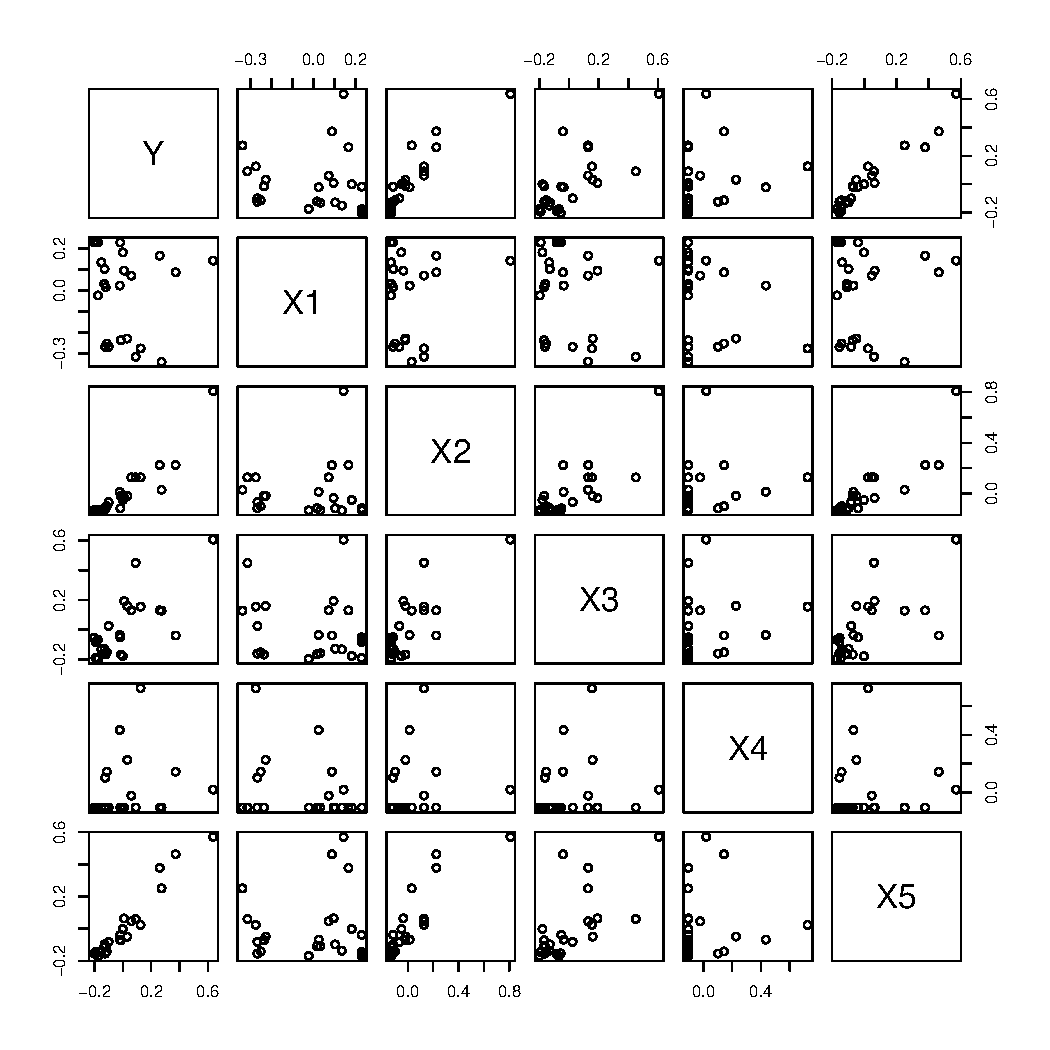
\includegraphics[width=\maxwidth]{figure/unnamed-chunk-1-1} 
\begin{kframe}\begin{alltt}
  \hlkwd{cor}\hlstd{(dat)}
\end{alltt}
\begin{verbatim}
##             Y          X1          X2         X3          X4         X5
## Y   1.0000000 -0.11453460  0.92345442  0.7413715  0.22497528 0.96813120
## X1 -0.1145346  1.00000000 -0.01415504 -0.1885895 -0.36265249 0.02700832
## X2  0.9234544 -0.01415504  1.00000000  0.8000696  0.22412565 0.87786360
## X3  0.7413715 -0.18858951  0.80006959  1.0000000  0.16609137 0.67269398
## X4  0.2249753 -0.36265249  0.22412565  0.1660914  1.00000000 0.08929658
## X5  0.9681312  0.02700832  0.87786360  0.6726940  0.08929658 1.00000000
\end{verbatim}
\end{kframe}
\end{knitrout}

\qquad We find that Y is highly correlated with X2, X3 and X5. and X2, X3 and X5 are highly correlated with each other, which means the multicollinearity is present.

\item

\begin{knitrout}
\definecolor{shadecolor}{rgb}{0.969, 0.969, 0.969}\color{fgcolor}\begin{kframe}
\begin{alltt}
  \hlkwd{require}\hlstd{(Matrix)}
\end{alltt}


{\ttfamily\noindent\itshape\color{messagecolor}{\#\# Loading required package: Matrix}}

{\ttfamily\noindent\color{warningcolor}{\#\# Warning: package 'Matrix' was built under R version 3.1.2}}\begin{alltt}
  \hlstd{X} \hlkwb{=} \hlstd{dat[,} \hlnum{2}\hlopt{:}\hlnum{6}\hlstd{]}
  \hlstd{X} \hlkwb{=} \hlkwd{as.matrix}\hlstd{(X)}
  \hlstd{P} \hlkwb{=} \hlkwd{t}\hlstd{(X)} \hlopt \hlstd{X}
  \hlkwd{eigen}\hlstd{(P)}
\end{alltt}
\begin{verbatim}
## $values
## [1] 2.63414515 1.33018568 0.65704211 0.29575194 0.08287513
## 
## $vectors
##            [,1]         [,2]        [,3]        [,4]        [,5]
## [1,] -0.1012189  0.720376426  0.63332131 -0.25097092  0.08203814
## [2,]  0.5913231  0.122265531  0.09155295  0.08619205 -0.78713218
## [3,]  0.5475583  0.004633543 -0.24983677 -0.73925733  0.30205730
## [4,]  0.1893656 -0.646792392  0.72651658 -0.06042441  0.11967806
## [5,]  0.5517357  0.218511047  0.01665599  0.61598053  0.51781389
\end{verbatim}
\end{kframe}
\end{knitrout}

\qquad Some eigenvalues are close to zero, so that it does exist multicollinearity.

\item

\begin{knitrout}
\definecolor{shadecolor}{rgb}{0.969, 0.969, 0.969}\color{fgcolor}\begin{kframe}
\begin{alltt}
  \hlstd{fit} \hlkwb{=} \hlkwd{lm}\hlstd{(Y} \hlopt{~} \hlnum{0} \hlopt{+} \hlstd{.,} \hlkwc{data} \hlstd{= dat)}
  \hlkwd{summary}\hlstd{(fit)}
\end{alltt}
\begin{verbatim}
## 
## Call:
## lm(formula = Y ~ 0 + ., data = dat)
## 
## Residuals:
##       Min        1Q    Median        3Q       Max 
## -0.052406 -0.016609 -0.004069  0.014375  0.070701 
## 
## Coefficients:
##    Estimate Std. Error t value Pr(>|t|)    
## X1 -0.10461    0.03556  -2.942  0.00807 ** 
## X2  0.24656    0.08636   2.855  0.00979 ** 
## X3  0.01854    0.05545   0.334  0.74159    
## X4  0.06294    0.03581   1.758  0.09410 .  
## X5  0.73642    0.06744  10.920 7.06e-10 ***
## ---
## Signif. codes:  0 '***' 0.001 '**' 0.01 '*' 0.05 '.' 0.1 ' ' 1
## 
## Residual standard error: 0.03121 on 20 degrees of freedom
## Multiple R-squared:  0.9805,	Adjusted R-squared:  0.9757 
## F-statistic: 201.4 on 5 and 20 DF,  p-value: < 2.2e-16
\end{verbatim}
\begin{alltt}
  \hlkwd{anova}\hlstd{(fit)}
\end{alltt}
\begin{verbatim}
## Analysis of Variance Table
## 
## Response: Y
##           Df  Sum Sq Mean Sq  F value    Pr(>F)    
## X1         1 0.01312 0.01312  13.4704  0.001519 ** 
## X2         1 0.84995 0.84995 872.7651 < 2.2e-16 ***
## X3         1 0.00073 0.00073   0.7458  0.398038    
## X4         1 0.00061 0.00061   0.6247  0.438588    
## X5         1 0.11612 0.11612 119.2409 7.064e-10 ***
## Residuals 20 0.01948 0.00097                       
## ---
## Signif. codes:  0 '***' 0.001 '**' 0.01 '*' 0.05 '.' 0.1 ' ' 1
\end{verbatim}
\end{kframe}
\end{knitrout}

\qquad In this multiple regression model, X1,X2, and X5 are more important to predict sale price.

\item
\begin{knitrout}
\definecolor{shadecolor}{rgb}{0.969, 0.969, 0.969}\color{fgcolor}\begin{kframe}
\begin{alltt}
  \hlkwd{require}\hlstd{(faraway)}
\end{alltt}


{\ttfamily\noindent\itshape\color{messagecolor}{\#\# Loading required package: faraway}}\begin{alltt}
  \hlkwd{vif}\hlstd{(fit)}
\end{alltt}


{\ttfamily\noindent\color{warningcolor}{\#\# Warning in vif.lm(fit): No intercept term detected.\ \ Results may surprise.}}\begin{verbatim}
##       X1       X2       X3       X4       X5 
## 1.298654 7.657888 3.157590 1.316618 4.670186
\end{verbatim}
\end{kframe}
\end{knitrout}

\qquad All VIF $>$1 shows that each X variable has the intercorrelation with the rest of the X variables.

\item

\begin{knitrout}
\definecolor{shadecolor}{rgb}{0.969, 0.969, 0.969}\color{fgcolor}\begin{kframe}
\begin{alltt}
  \hlkwd{library}\hlstd{(}\hlstr{'MASS'}\hlstd{)}
\end{alltt}


{\ttfamily\noindent\color{warningcolor}{\#\# Warning: package 'MASS' was built under R version 3.1.2}}\begin{alltt}
  \hlkwd{select}\hlstd{(}\hlkwd{lm.ridge}\hlstd{(Y} \hlopt{~} \hlnum{0} \hlopt{+} \hlstd{.,} \hlkwc{data} \hlstd{= dat,}
                \hlkwc{lambda} \hlstd{=} \hlkwd{seq}\hlstd{(}\hlnum{0}\hlstd{,} \hlnum{1}\hlstd{,} \hlnum{.001}\hlstd{)))}
\end{alltt}
\begin{verbatim}
## modified HKB estimator is 0.1181183 
## modified L-W estimator is 0.07448998 
## smallest value of GCV  at 0.321
\end{verbatim}
\begin{alltt}
  \hlstd{k} \hlkwb{=} \hlnum{.321}
  \hlkwd{require}\hlstd{(}\hlstr{'ridge'}\hlstd{)}
\end{alltt}


{\ttfamily\noindent\itshape\color{messagecolor}{\#\# Loading required package: ridge}}

{\ttfamily\noindent\color{warningcolor}{\#\# Warning: package 'ridge' was built under R version 3.1.2}}\begin{alltt}
  \hlstd{model} \hlkwb{=} \hlkwd{linearRidge}\hlstd{(Y} \hlopt{~} \hlnum{0} \hlopt{+} \hlstd{.,} \hlkwc{data} \hlstd{= dat,}
                    \hlkwc{lambda} \hlstd{= k,} \hlkwc{scaling} \hlstd{=} \hlstr{'none'}\hlstd{); model}
\end{alltt}
\begin{verbatim}
## 
## Call:
## linearRidge(formula = Y ~ 0 + ., data = dat, lambda = k, scaling = "none")
## 
##          X1          X2          X3          X4          X5 
## -0.06004494  0.30522205  0.12451487  0.05500698  0.46414629
\end{verbatim}
\begin{alltt}
  \hlkwd{summary}\hlstd{(model)}
\end{alltt}
\begin{verbatim}
## 
## Call:
## linearRidge(formula = Y ~ 0 + ., data = dat, lambda = k, scaling = "none")
## 
## 
## Coefficients:
##    Estimate Std. Error t value Pr(>|t|)    
## X1 -0.06004    0.03763   1.596  0.11060    
## X2  0.30522    0.03263   9.355  < 2e-16 ***
## X3  0.12451    0.03829   3.252  0.00114 ** 
## X4  0.05501    0.03774   1.457  0.14501    
## X5  0.46415    0.03640  12.751  < 2e-16 ***
## ---
## Signif. codes:  0 '***' 0.001 '**' 0.01 '*' 0.05 '.' 0.1 ' ' 1
## 
## Ridge parameter: 0.321
## 
## Degrees of freedom: model 3.053 , variance 2.167 , residual 3.94
\end{verbatim}
\end{kframe}
\end{knitrout}

\qquad Parameter estimates and their standard errors are shown in the summary(model).

\item

\begin{knitrout}
\definecolor{shadecolor}{rgb}{0.969, 0.969, 0.969}\color{fgcolor}\begin{kframe}
\begin{alltt}
  \hlkwd{plot}\hlstd{(X}\hlopt\hlstd{model}\hlopt{$}\hlstd{coef, model}\hlopt{$}\hlstd{y)}
\end{alltt}
\end{kframe}
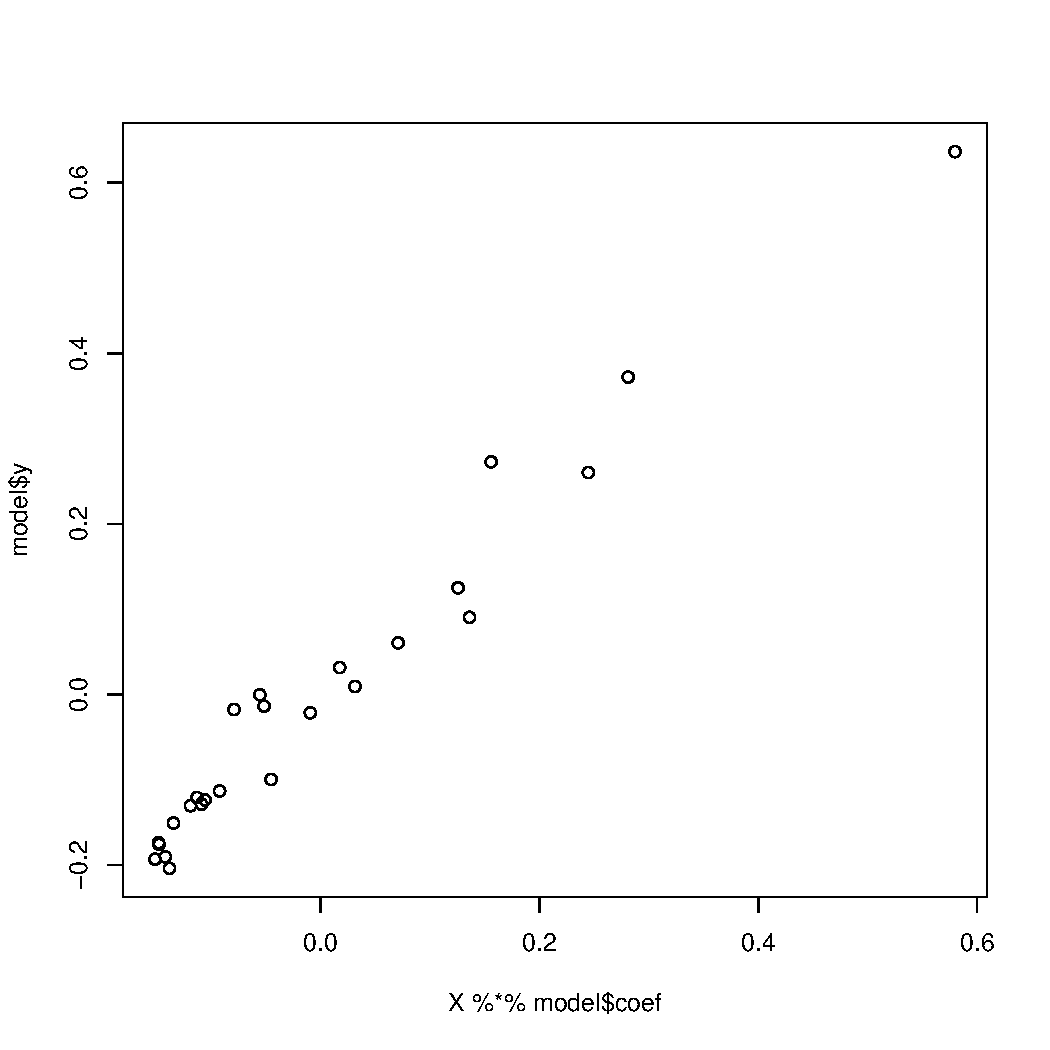
\includegraphics[width=\maxwidth]{figure/unnamed-chunk-6-1} 
\begin{kframe}\begin{alltt}
  \hlkwd{par}\hlstd{(} \hlkwc{mfrow} \hlstd{=} \hlkwd{c}\hlstd{(}\hlnum{1}\hlstd{,} \hlnum{2}\hlstd{))}
  \hlkwd{plot}\hlstd{(X}\hlopt\hlstd{model}\hlopt{$}\hlstd{coef, model}\hlopt{$}\hlstd{y} \hlopt{-} \hlstd{X}\hlopt\hlstd{model}\hlopt{$}\hlstd{coef)}
  \hlkwd{qqnorm}\hlstd{(model}\hlopt{$}\hlstd{y} \hlopt{-} \hlstd{X}\hlopt\hlstd{model}\hlopt{$}\hlstd{coef)}
  \hlkwd{qqline}\hlstd{(model}\hlopt{$}\hlstd{y} \hlopt{-} \hlstd{X}\hlopt\hlstd{model}\hlopt{$}\hlstd{coef)}
\end{alltt}
\end{kframe}
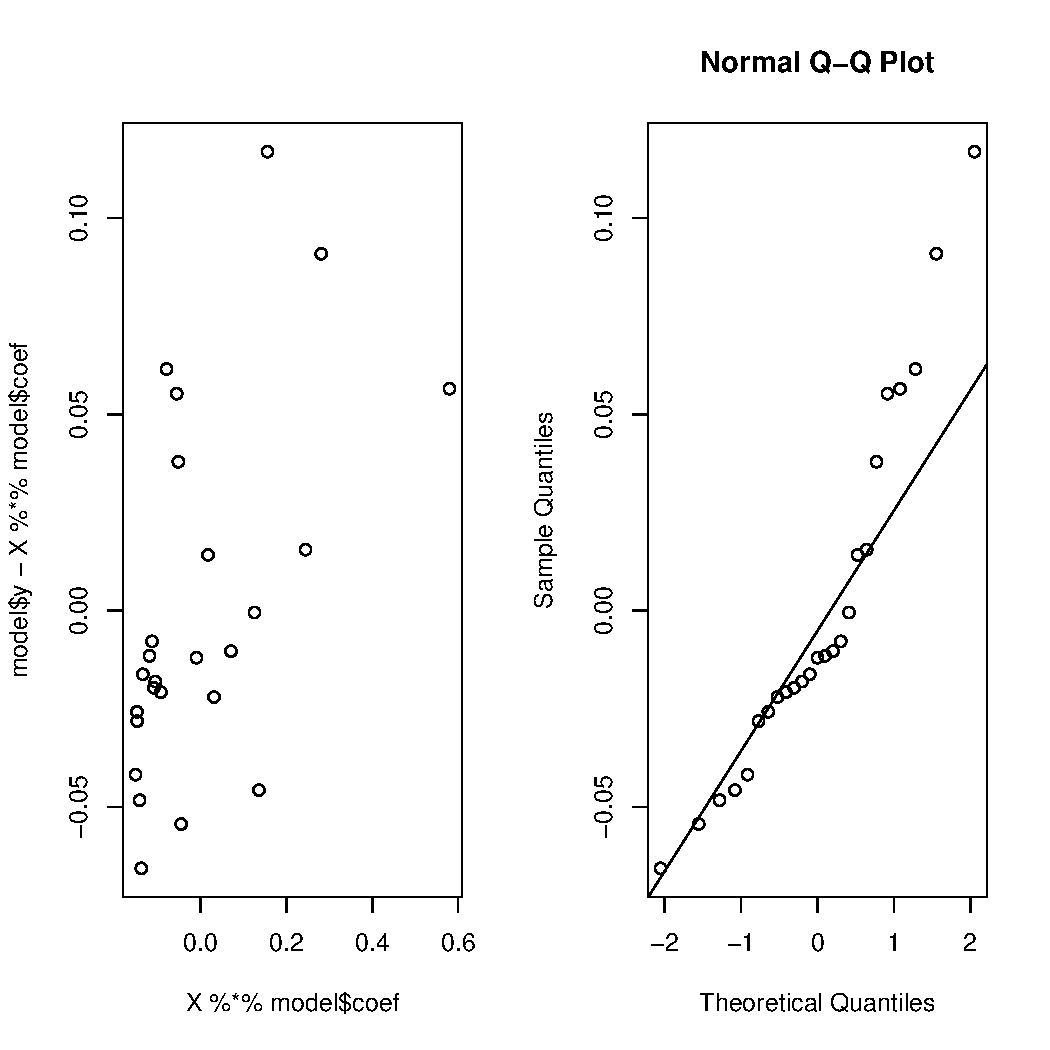
\includegraphics[width=\maxwidth]{figure/unnamed-chunk-6-2} 

\end{knitrout}

\qquad The residuals versus fitted values plots shows no sign for unequal variance.And the QQ-plot indicates approximately normal distribution with heavy tail, so that normality assumption seems to be reasonable, we can use model here.

\item

\begin{knitrout}
\definecolor{shadecolor}{rgb}{0.969, 0.969, 0.969}\color{fgcolor}\begin{kframe}
\begin{alltt}
  \hlstd{ans} \hlkwb{=} \hlkwd{solve}\hlstd{(P} \hlopt{+} \hlkwd{diag}\hlstd{(k,}\hlnum{5}\hlstd{,}\hlnum{5}\hlstd{))} \hlopt \hlstd{P} \hlopt \hlkwd{solve}\hlstd{(P} \hlopt{+} \hlkwd{diag}\hlstd{(k,}\hlnum{5}\hlstd{,}\hlnum{5}\hlstd{))}
  \hlkwd{diag}\hlstd{(ans)}
\end{alltt}
\begin{verbatim}
##        X1        X2        X3        X4        X5 
## 0.5841713 0.4390908 0.6045876 0.5875868 0.5465513
\end{verbatim}
\end{kframe}
\end{knitrout}

\qquad VIF of the estimated ridge regression are shown in the above. All VIF are smaller than 1, which means they have little intercorrelation between X variables.

\end{enumerate}

\section{2}

\begin{enumerate}[(a)]

\item

\begin{knitrout}
\definecolor{shadecolor}{rgb}{0.969, 0.969, 0.969}\color{fgcolor}\begin{kframe}
\begin{alltt}
  \hlkwd{require}\hlstd{(gdata)}
  \hlstd{dat} \hlkwb{=} \hlkwd{read.xls}\hlstd{(}\hlstr{"ratdrink.xlsx"}\hlstd{)}
  \hlstd{dat} \hlkwb{=} \hlstd{dat[,} \hlnum{1}\hlopt{:}\hlnum{4}\hlstd{]}
  \hlstd{dat}\hlopt{$}\hlstd{wk} \hlkwb{=} \hlstd{dat}\hlopt{$}\hlstd{weeks} \hlopt{-} \hlkwd{mean}\hlstd{(dat}\hlopt{$}\hlstd{weeks); dat}\hlopt{$}\hlstd{wk}
\end{alltt}
\begin{verbatim}
##   [1] -2 -1  0  1  2 -2 -1  0  1  2 -2 -1  0  1  2 -2 -1  0  1  2 -2 -1  0
##  [24]  1  2 -2 -1  0  1  2 -2 -1  0  1  2 -2 -1  0  1  2 -2 -1  0  1  2 -2
##  [47] -1  0  1  2 -2 -1  0  1  2 -2 -1  0  1  2 -2 -1  0  1  2 -2 -1  0  1
##  [70]  2 -2 -1  0  1  2 -2 -1  0  1  2 -2 -1  0  1  2 -2 -1  0  1  2 -2 -1
##  [93]  0  1  2 -2 -1  0  1  2 -2 -1  0  1  2 -2 -1  0  1  2 -2 -1  0  1  2
## [116] -2 -1  0  1  2 -2 -1  0  1  2 -2 -1  0  1  2 -2 -1  0  1  2
\end{verbatim}
\begin{alltt}
  \hlstd{dat}\hlopt{$}\hlstd{wk2} \hlkwb{=} \hlstd{dat}\hlopt{$}\hlstd{wk}\hlopt{^}\hlnum{2}\hlstd{; dat}\hlopt{$}\hlstd{wk2}
\end{alltt}
\begin{verbatim}
##   [1] 4 1 0 1 4 4 1 0 1 4 4 1 0 1 4 4 1 0 1 4 4 1 0 1 4 4 1 0 1 4 4 1 0 1 4
##  [36] 4 1 0 1 4 4 1 0 1 4 4 1 0 1 4 4 1 0 1 4 4 1 0 1 4 4 1 0 1 4 4 1 0 1 4
##  [71] 4 1 0 1 4 4 1 0 1 4 4 1 0 1 4 4 1 0 1 4 4 1 0 1 4 4 1 0 1 4 4 1 0 1 4
## [106] 4 1 0 1 4 4 1 0 1 4 4 1 0 1 4 4 1 0 1 4 4 1 0 1 4 4 1 0 1 4
\end{verbatim}
\begin{alltt}
  \hlstd{dat}\hlopt{$}\hlstd{weeks} \hlkwb{=} \hlkwd{as.factor}\hlstd{(dat}\hlopt{$}\hlstd{weeks)}
  \hlstd{dat}\hlopt{$}\hlstd{subject} \hlkwb{=} \hlkwd{as.factor}\hlstd{(dat}\hlopt{$}\hlstd{subject)}
  \hlstd{datt} \hlkwb{=} \hlkwd{split}\hlstd{(dat, dat}\hlopt{$}\hlstd{treat)}
  \hlkwd{par}\hlstd{(}\hlkwc{mfrow} \hlstd{=} \hlkwd{c}\hlstd{(}\hlnum{1}\hlstd{,} \hlnum{3}\hlstd{))}
  \hlkwd{sapply}\hlstd{(datt,} \hlkwa{function}\hlstd{(}\hlkwc{x}\hlstd{)\{}\hlkwd{interaction.plot}\hlstd{(x}\hlopt{$}\hlstd{weeks, x}\hlopt{$}\hlstd{subject, x}\hlopt{$}\hlstd{weight,}
                                            \hlkwc{ylim} \hlstd{=} \hlkwd{c}\hlstd{(}\hlnum{40}\hlstd{,} \hlnum{200}\hlstd{),} \hlkwc{xlab} \hlstd{=} \hlkwd{unique}\hlstd{(x}\hlopt{$}\hlstd{treat))\})}
\end{alltt}
\end{kframe}
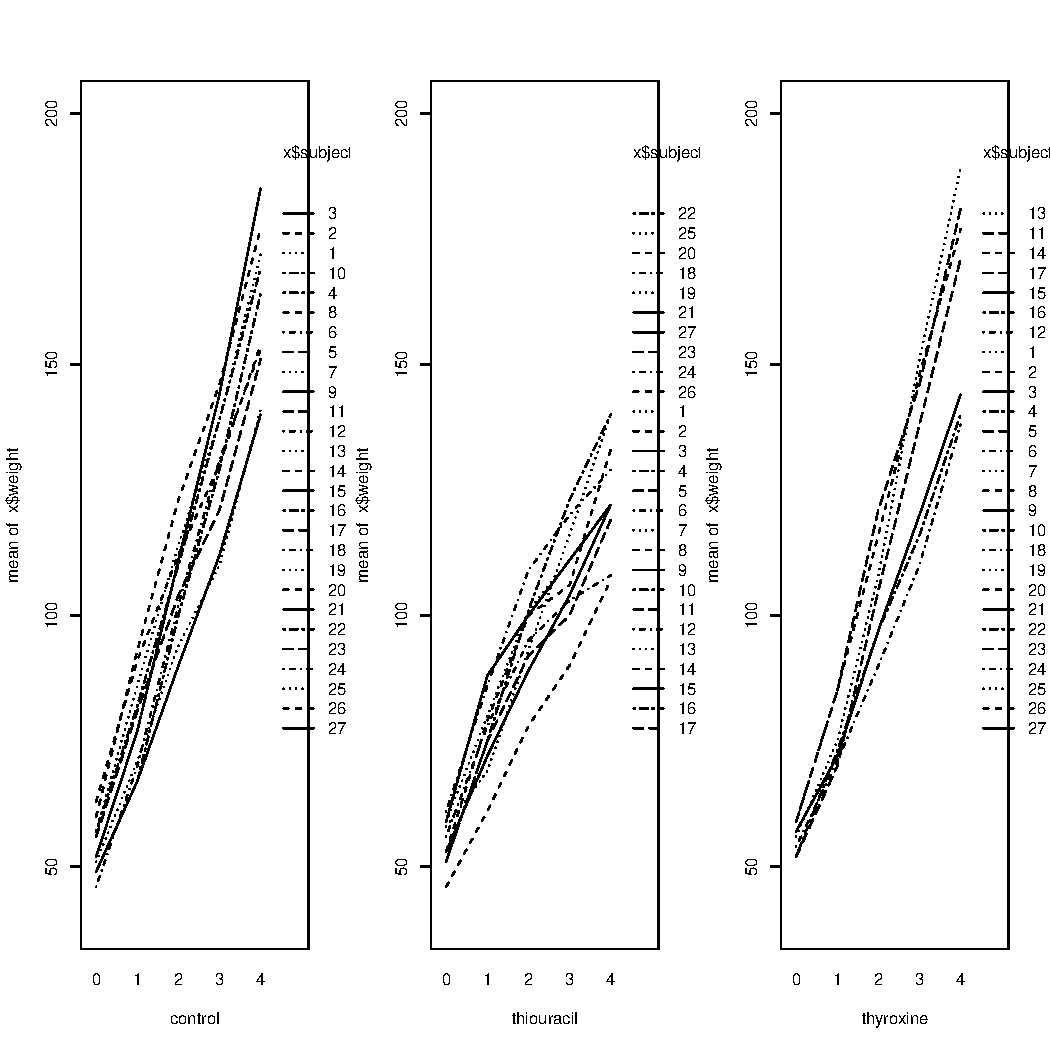
\includegraphics[width=\maxwidth]{figure/unnamed-chunk-8-1} 
\begin{kframe}\begin{verbatim}
## $control
## NULL
## 
## $thiouracil
## NULL
## 
## $thyroxine
## NULL
\end{verbatim}
\end{kframe}
\end{knitrout}

\item

\begin{knitrout}
\definecolor{shadecolor}{rgb}{0.969, 0.969, 0.969}\color{fgcolor}\begin{kframe}
\begin{alltt}
  \hlkwd{par}\hlstd{(}\hlkwc{mfrow} \hlstd{=} \hlkwd{c}\hlstd{(}\hlnum{1}\hlstd{,} \hlnum{1}\hlstd{))}
  \hlkwd{boxplot}\hlstd{(weight} \hlopt{~} \hlkwd{factor}\hlstd{(weeks)}\hlopt{*}\hlstd{treat,} \hlkwc{data} \hlstd{= dat)}
\end{alltt}
\end{kframe}
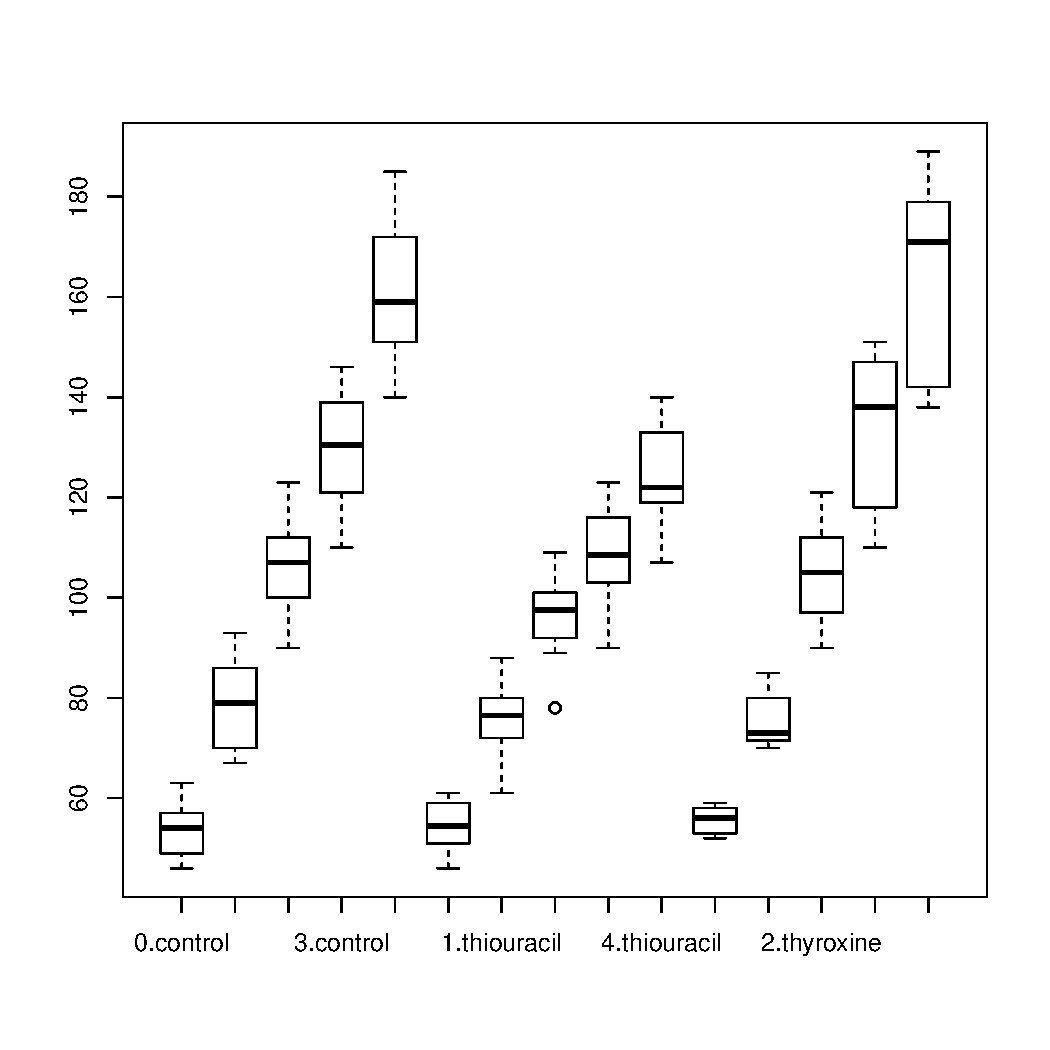
\includegraphics[width=\maxwidth]{figure/unnamed-chunk-9-1} 

\end{knitrout}

\qquad The mean weight becomes larger over time. And the variability of weight change over time gets bigger, treatment thyroxine has the biggest variability over time.

\item

\begin{knitrout}
\definecolor{shadecolor}{rgb}{0.969, 0.969, 0.969}\color{fgcolor}\begin{kframe}
\begin{alltt}
  \hlkwd{require}\hlstd{(lme4)}
\end{alltt}


{\ttfamily\noindent\itshape\color{messagecolor}{\#\# Loading required package: lme4}}

{\ttfamily\noindent\color{warningcolor}{\#\# Warning: package 'lme4' was built under R version 3.1.2}}

{\ttfamily\noindent\itshape\color{messagecolor}{\#\# Loading required package: Rcpp}}

{\ttfamily\noindent\color{warningcolor}{\#\# Warning: package 'Rcpp' was built under R version 3.1.2}}\begin{alltt}
  \hlstd{fit} \hlkwb{=} \hlkwd{lmer}\hlstd{(weight} \hlopt{~} \hlkwd{factor}\hlstd{(weeks)} \hlopt{+} \hlstd{treat} \hlopt{+} \hlkwd{factor}\hlstd{(weeks)}\hlopt{:}\hlstd{treat} \hlopt{+} \hlstd{(}\hlnum{1}\hlopt{|}\hlstd{subject),} \hlkwc{data} \hlstd{= dat )}
  \hlkwd{par}\hlstd{(}\hlkwc{mfrow} \hlstd{=} \hlkwd{c}\hlstd{(}\hlnum{1}\hlstd{,} \hlnum{1}\hlstd{))}
  \hlkwd{plot}\hlstd{(dat}\hlopt{$}\hlstd{weight,} \hlkwd{fitted}\hlstd{(fit))}
\end{alltt}
\end{kframe}
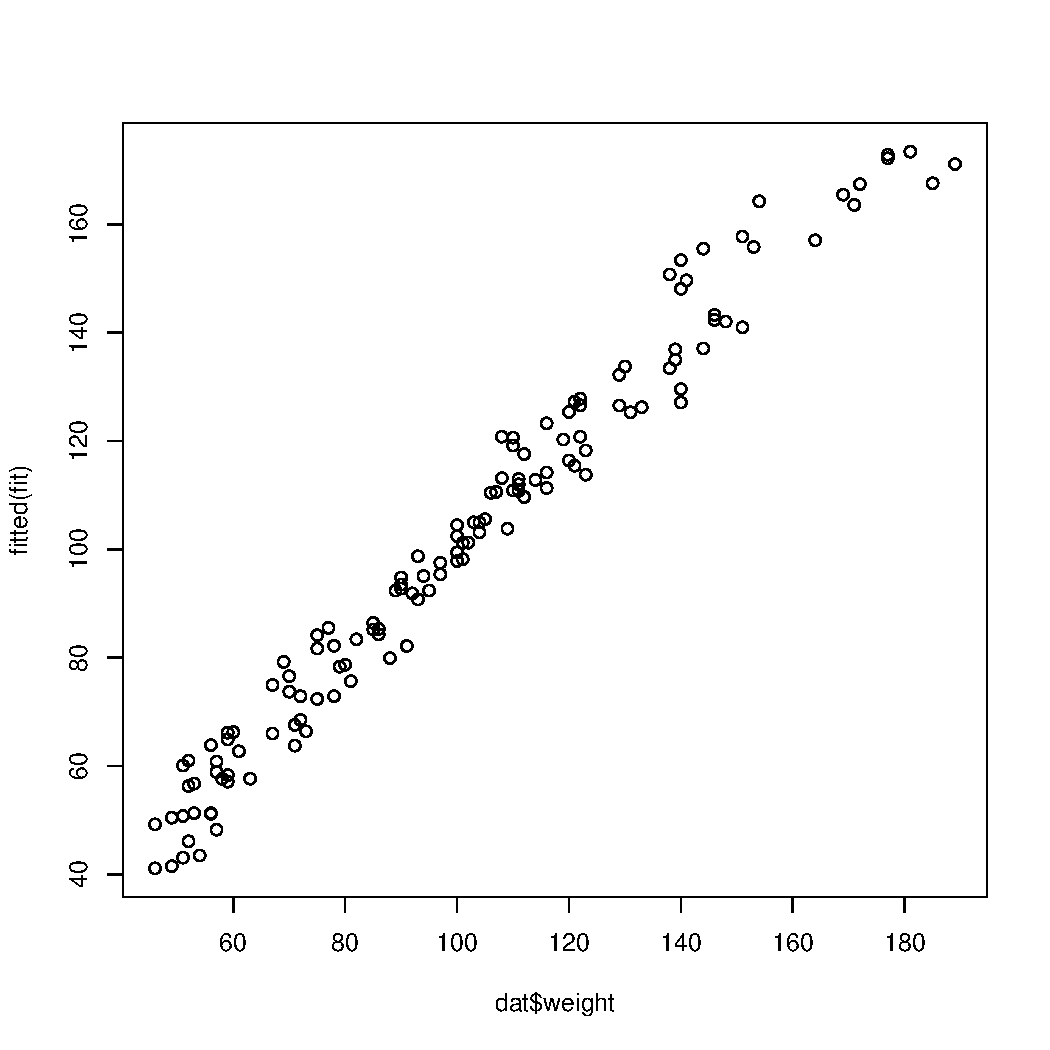
\includegraphics[width=\maxwidth]{figure/unnamed-chunk-10-1} 
\begin{kframe}\begin{alltt}
  \hlkwd{plot}\hlstd{(fit,} \hlkwc{which} \hlstd{=} \hlnum{1}\hlstd{)}
\end{alltt}
\end{kframe}
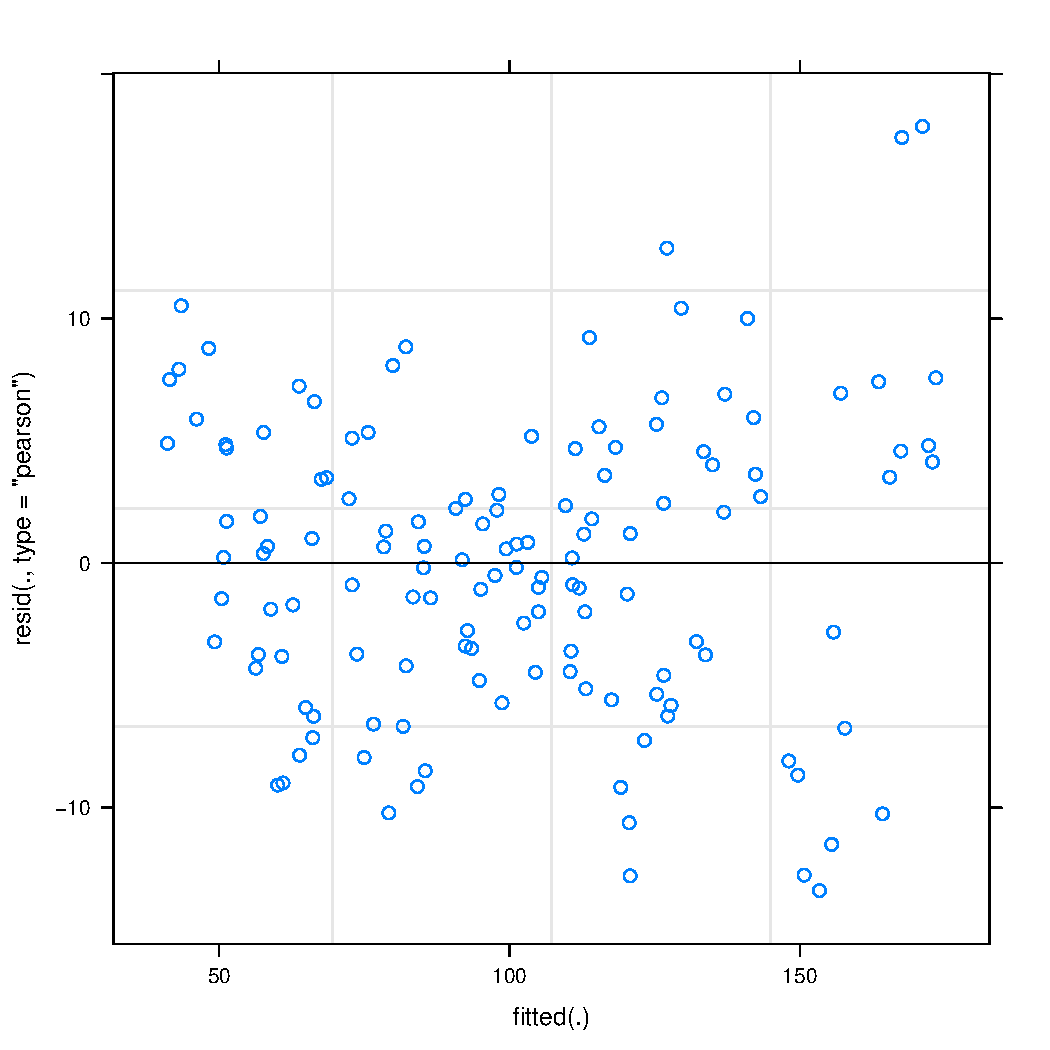
\includegraphics[width=\maxwidth]{figure/unnamed-chunk-10-2} 
\begin{kframe}\begin{alltt}
  \hlkwd{par}\hlstd{(}\hlkwc{mfrow} \hlstd{=} \hlkwd{c}\hlstd{(}\hlnum{1}\hlstd{,} \hlnum{1}\hlstd{))}
  \hlkwd{boxplot}\hlstd{(weight} \hlopt{~} \hlstd{weeks}\hlopt{*}\hlstd{treat,} \hlkwc{data} \hlstd{= dat)}
\end{alltt}
\end{kframe}
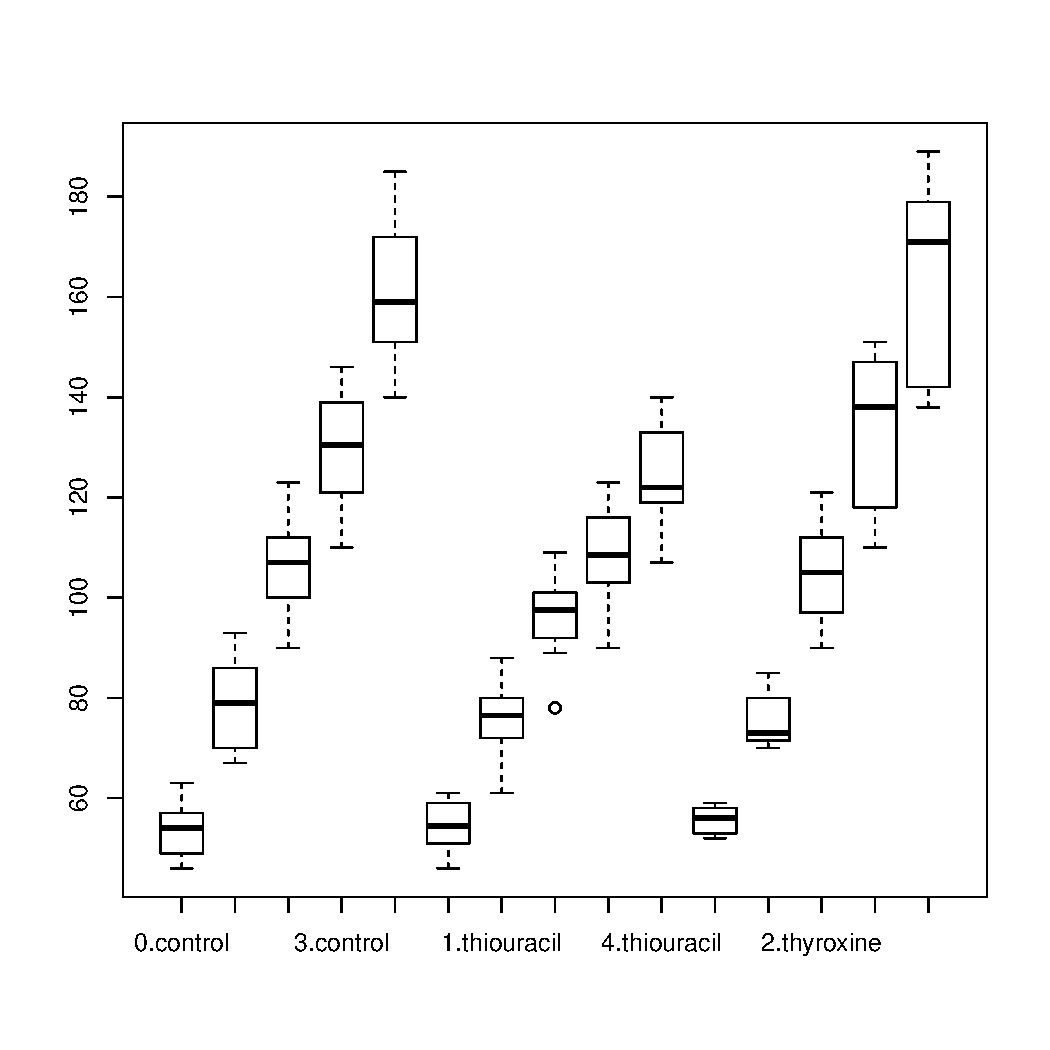
\includegraphics[width=\maxwidth]{figure/unnamed-chunk-10-3} 

\end{knitrout}

\qquad The residuals versus fitted values plots shows no sign for unequal variance.

\item

\begin{knitrout}
\definecolor{shadecolor}{rgb}{0.969, 0.969, 0.969}\color{fgcolor}\begin{kframe}
\begin{alltt}
  \hlkwd{summary}\hlstd{(fit)}
\end{alltt}
\begin{verbatim}
## Linear mixed model fit by REML ['lmerMod']
## Formula: 
## weight ~ factor(weeks) + treat + factor(weeks):treat + (1 | subject)
##    Data: dat
## 
## REML criterion at convergence: 892.1
## 
## Scaled residuals: 
##      Min       1Q   Median       3Q      Max 
## -1.90369 -0.60408  0.03345  0.64957  2.53828 
## 
## Random effects:
##  Groups   Name        Variance Std.Dev.
##  subject  (Intercept) 71.55    8.459   
##  Residual             49.51    7.036   
## Number of obs: 135, groups:  subject, 27
## 
## Fixed effects:
##                                Estimate Std. Error t value
## (Intercept)                     54.0000     3.4794   15.52
## factor(weeks)1                  24.5000     3.1468    7.79
## factor(weeks)2                  52.0000     3.1468   16.52
## factor(weeks)3                  76.1000     3.1468   24.18
## factor(weeks)4                 106.6000     3.1468   33.88
## treatthiouracil                  0.7000     4.9206    0.14
## treatthyroxine                   1.5714     5.4222    0.29
## factor(weeks)1:treatthiouracil  -2.9000     4.4503   -0.65
## factor(weeks)2:treatthiouracil -10.9000     4.4503   -2.45
## factor(weeks)3:treatthiouracil -22.4000     4.4503   -5.03
## factor(weeks)4:treatthiouracil -37.1000     4.4503   -8.34
## factor(weeks)1:treatthyroxine   -4.2143     4.9039   -0.86
## factor(weeks)2:treatthyroxine   -2.7143     4.9039   -0.55
## factor(weeks)3:treatthyroxine    1.0429     4.9039    0.21
## factor(weeks)4:treatthyroxine    0.6857     4.9039    0.14
## 
## Correlation of Fixed Effects:
##                   (Intr) fct()1 fct()2 fct()3 fct()4 trtthr trtthy
## factr(wks)1       -0.452                                          
## factr(wks)2       -0.452  0.500                                   
## factr(wks)3       -0.452  0.500  0.500                            
## factr(wks)4       -0.452  0.500  0.500  0.500                     
## treatthircl       -0.707  0.320  0.320  0.320  0.320              
## treatthyrxn       -0.642  0.290  0.290  0.290  0.290  0.454       
## fctr(wks)1:trtthr  0.320 -0.707 -0.354 -0.354 -0.354 -0.452 -0.205
## fctr(wks)2:trtthr  0.320 -0.354 -0.707 -0.354 -0.354 -0.452 -0.205
## fctr(wks)3:trtthr  0.320 -0.354 -0.354 -0.707 -0.354 -0.452 -0.205
## fctr(wks)4:trtthr  0.320 -0.354 -0.354 -0.354 -0.707 -0.452 -0.205
## fctr(wks)1:trtthy  0.290 -0.642 -0.321 -0.321 -0.321 -0.205 -0.452
## fctr(wks)2:trtthy  0.290 -0.321 -0.642 -0.321 -0.321 -0.205 -0.452
## fctr(wks)3:trtthy  0.290 -0.321 -0.321 -0.642 -0.321 -0.205 -0.452
## fctr(wks)4:trtthy  0.290 -0.321 -0.321 -0.321 -0.642 -0.205 -0.452
##                   fctr(wks)1:trtthr fctr(wks)2:trtthr fctr(wks)3:trtthr
## factr(wks)1                                                            
## factr(wks)2                                                            
## factr(wks)3                                                            
## factr(wks)4                                                            
## treatthircl                                                            
## treatthyrxn                                                            
## fctr(wks)1:trtthr                                                      
## fctr(wks)2:trtthr  0.500                                               
## fctr(wks)3:trtthr  0.500             0.500                             
## fctr(wks)4:trtthr  0.500             0.500             0.500           
## fctr(wks)1:trtthy  0.454             0.227             0.227           
## fctr(wks)2:trtthy  0.227             0.454             0.227           
## fctr(wks)3:trtthy  0.227             0.227             0.454           
## fctr(wks)4:trtthy  0.227             0.227             0.227           
##                   fctr(wks)4:trtthr fctr(wks)1:trtthy fctr(wks)2:trtthy
## factr(wks)1                                                            
## factr(wks)2                                                            
## factr(wks)3                                                            
## factr(wks)4                                                            
## treatthircl                                                            
## treatthyrxn                                                            
## fctr(wks)1:trtthr                                                      
## fctr(wks)2:trtthr                                                      
## fctr(wks)3:trtthr                                                      
## fctr(wks)4:trtthr                                                      
## fctr(wks)1:trtthy  0.227                                               
## fctr(wks)2:trtthy  0.227             0.500                             
## fctr(wks)3:trtthy  0.227             0.500             0.500           
## fctr(wks)4:trtthy  0.454             0.500             0.500           
##                   fctr(wks)3:trtthy
## factr(wks)1                        
## factr(wks)2                        
## factr(wks)3                        
## factr(wks)4                        
## treatthircl                        
## treatthyrxn                        
## fctr(wks)1:trtthr                  
## fctr(wks)2:trtthr                  
## fctr(wks)3:trtthr                  
## fctr(wks)4:trtthr                  
## fctr(wks)1:trtthy                  
## fctr(wks)2:trtthy                  
## fctr(wks)3:trtthy                  
## fctr(wks)4:trtthy  0.500
\end{verbatim}
\begin{alltt}
  \hlkwd{anova}\hlstd{(fit)}
\end{alltt}
\begin{verbatim}
## Analysis of Variance Table
##                     Df Sum Sq Mean Sq  F value
## factor(weeks)        4 145188   36297 733.0981
## treat                2    770     385   7.7774
## factor(weeks):treat  8   6403     800  16.1641
\end{verbatim}
\begin{alltt}
  \hlstd{fit1} \hlkwb{=} \hlkwd{lm}\hlstd{(weight} \hlopt{~} \hlkwd{factor}\hlstd{(weeks)} \hlopt{+} \hlstd{treat} \hlopt{+} \hlkwd{factor}\hlstd{(weeks)}\hlopt{:}\hlstd{treat,} \hlkwc{data} \hlstd{= dat )}
  \hlstd{fit2} \hlkwb{=} \hlkwd{lmer}\hlstd{(weight} \hlopt{~} \hlstd{treat} \hlopt{+} \hlkwd{factor}\hlstd{(weeks)}\hlopt{:}\hlstd{treat} \hlopt{+} \hlstd{(}\hlnum{1}\hlopt{|}\hlstd{subject),} \hlkwc{data} \hlstd{= dat )}
  \hlstd{fit3} \hlkwb{=} \hlkwd{lmer}\hlstd{(weight} \hlopt{~} \hlkwd{factor}\hlstd{(weeks)} \hlopt{+} \hlkwd{factor}\hlstd{(weeks)}\hlopt{:}\hlstd{treat} \hlopt{+} \hlstd{(}\hlnum{1}\hlopt{|}\hlstd{subject),} \hlkwc{data} \hlstd{= dat )}
  \hlstd{fit4} \hlkwb{=} \hlkwd{lmer}\hlstd{(weight} \hlopt{~} \hlkwd{factor}\hlstd{(weeks)} \hlopt{+} \hlstd{treat} \hlopt{+} \hlstd{(}\hlnum{1}\hlopt{|}\hlstd{subject),} \hlkwc{data} \hlstd{= dat )}
  \hlkwd{AIC}\hlstd{(fit)}
\end{alltt}
\begin{verbatim}
## [1] 926.1398
\end{verbatim}
\begin{alltt}
  \hlkwd{AIC}\hlstd{(fit1)}
\end{alltt}
\begin{verbatim}
## [1] 1046.712
\end{verbatim}
\begin{alltt}
  \hlkwd{AIC}\hlstd{(fit2)}
\end{alltt}
\begin{verbatim}
## [1] 926.1398
\end{verbatim}
\begin{alltt}
  \hlkwd{AIC}\hlstd{(fit3)}
\end{alltt}
\begin{verbatim}
## [1] 926.1398
\end{verbatim}
\begin{alltt}
  \hlkwd{AIC}\hlstd{(fit4)}
\end{alltt}
\begin{verbatim}
## [1] 1034.661
\end{verbatim}
\end{kframe}
\end{knitrout}

\qquad The AIC of the full model is 926.1398, which means it's the smallest AIC of all. So there's no need to drop the terms.

\end{enumerate}

\section{3}

\begin{enumerate}[(a)]

\item

\begin{knitrout}
\definecolor{shadecolor}{rgb}{0.969, 0.969, 0.969}\color{fgcolor}\begin{kframe}
\begin{alltt}
  \hlstd{model} \hlkwb{=} \hlkwd{lmer}\hlstd{(weight} \hlopt{~} \hlstd{wk} \hlopt{+} \hlstd{treat}  \hlopt{+} \hlstd{(}\hlnum{1}\hlopt{|}\hlstd{subject)} \hlopt{+} \hlstd{(}\hlnum{0} \hlopt{+} \hlstd{wk}\hlopt{|}\hlstd{subject),} \hlkwc{data} \hlstd{= dat)}
  \hlkwd{par}\hlstd{(} \hlkwc{mfrow} \hlstd{=} \hlkwd{c}\hlstd{(}\hlnum{1}\hlstd{,} \hlnum{1}\hlstd{))}
  \hlkwd{plot}\hlstd{(model,} \hlkwc{which} \hlstd{=} \hlnum{1}\hlstd{)}
\end{alltt}
\end{kframe}
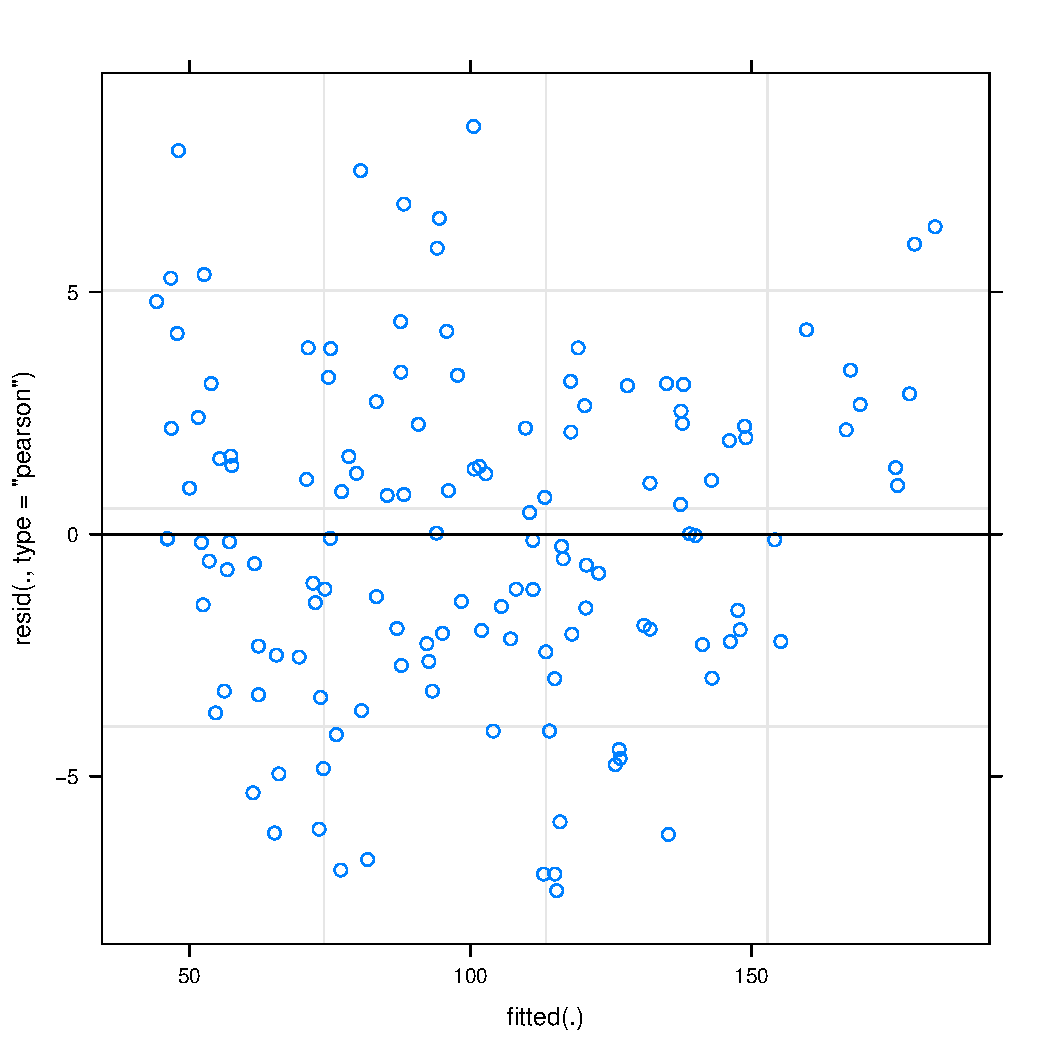
\includegraphics[width=\maxwidth]{figure/unnamed-chunk-12-1} 
\begin{kframe}\begin{alltt}
  \hlkwd{hist}\hlstd{(}\hlkwd{resid}\hlstd{(model))}
\end{alltt}
\end{kframe}
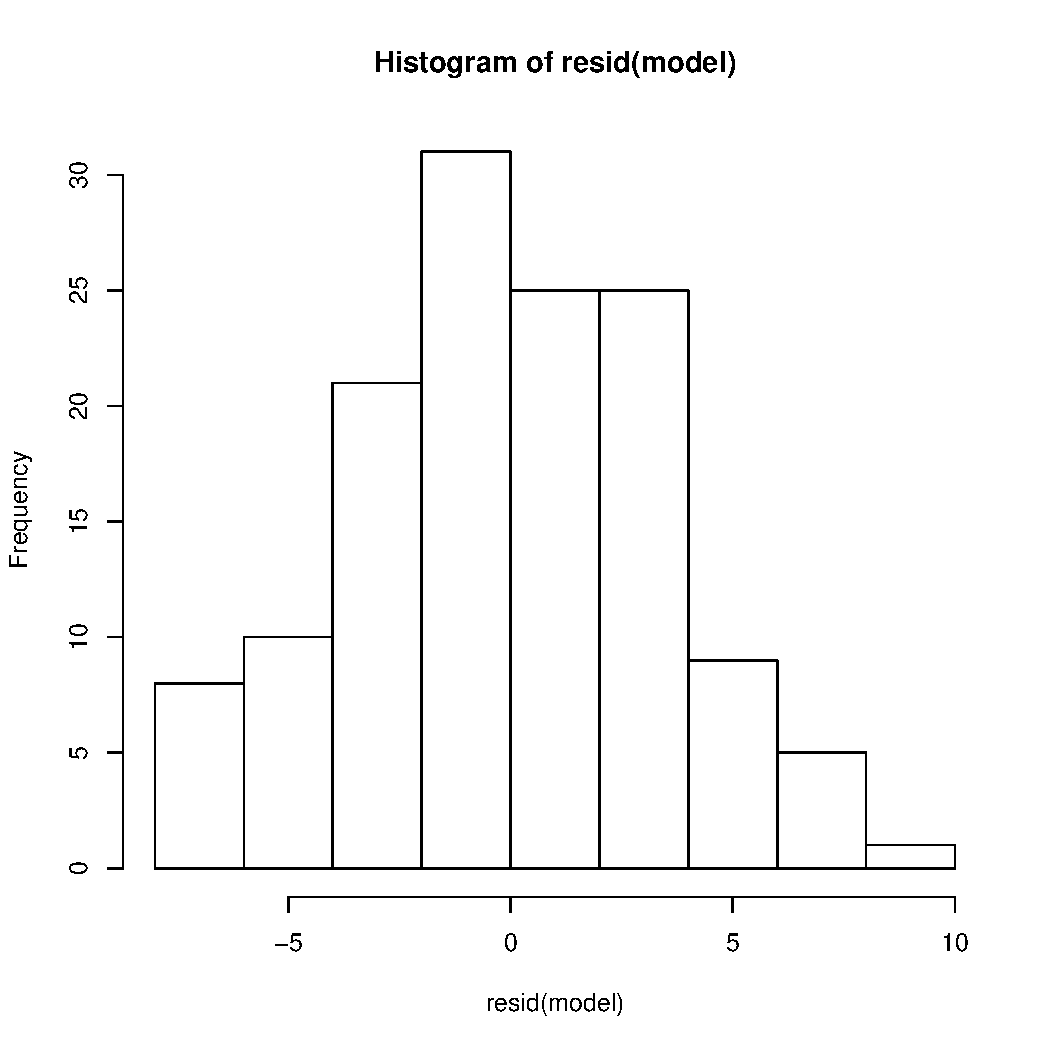
\includegraphics[width=\maxwidth]{figure/unnamed-chunk-12-2} 
\begin{kframe}\begin{alltt}
  \hlkwd{boxplot}\hlstd{(weight} \hlopt{~} \hlstd{wk}\hlopt{*}\hlstd{treat,} \hlkwc{data} \hlstd{= dat)}
\end{alltt}
\end{kframe}
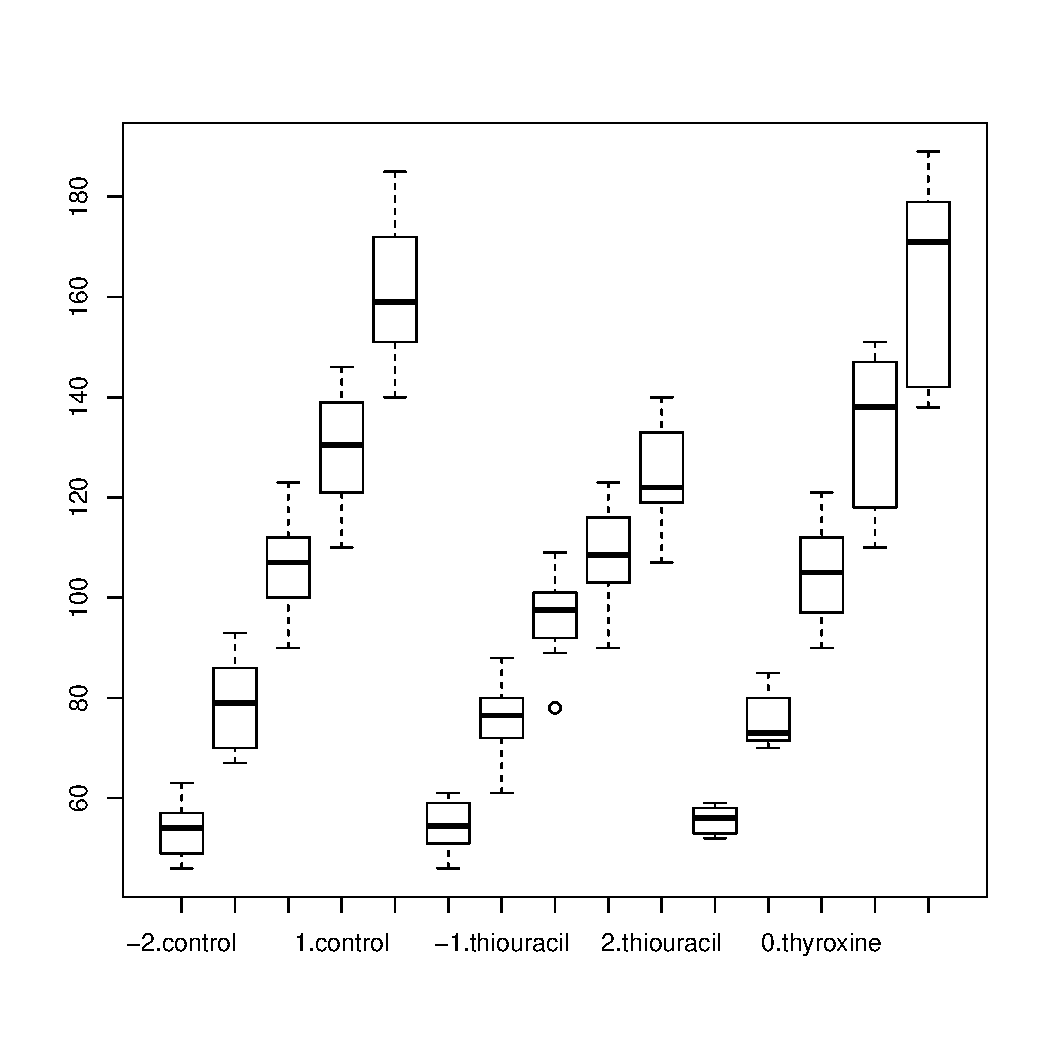
\includegraphics[width=\maxwidth]{figure/unnamed-chunk-12-3} 

\end{knitrout}

\item

\begin{knitrout}
\definecolor{shadecolor}{rgb}{0.969, 0.969, 0.969}\color{fgcolor}\begin{kframe}
\begin{alltt}
  \hlstd{model2} \hlkwb{=} \hlkwd{lmer}\hlstd{(weight} \hlopt{~} \hlstd{wk} \hlopt{+} \hlstd{wk2} \hlopt{+} \hlstd{treat}  \hlopt{+} \hlstd{(}\hlnum{1}\hlopt{|}\hlstd{subject)}\hlopt{+} \hlstd{(}\hlnum{0} \hlopt{+} \hlstd{wk}\hlopt{|}\hlstd{subject)}\hlopt{+} \hlstd{(}\hlnum{0} \hlopt{+} \hlstd{wk2}\hlopt{|}\hlstd{subject),} \hlkwc{data} \hlstd{= dat )}
  \hlkwd{summary}\hlstd{(model2)}
\end{alltt}
\begin{verbatim}
## Linear mixed model fit by REML ['lmerMod']
## Formula: weight ~ wk + wk2 + treat + (1 | subject) + (0 + wk | subject) +  
##     (0 + wk2 | subject)
##    Data: dat
## 
## REML criterion at convergence: 908.3
## 
## Scaled residuals: 
##     Min      1Q  Median      3Q     Max 
## -2.4904 -0.4034  0.0611  0.3895  1.7395 
## 
## Random effects:
##  Groups    Name        Variance Std.Dev.
##  subject   (Intercept) 87.138   9.335   
##  subject.1 wk          36.444   6.037   
##  subject.2 wk2          2.042   1.429   
##  Residual               9.402   3.066   
## Number of obs: 135, groups:  subject, 27
## 
## Fixed effects:
##                  Estimate Std. Error t value
## (Intercept)     104.87487    3.02136   34.71
## wk               23.18148    1.17669   19.70
## wk2               0.08201    0.31704    0.26
## treatthiouracil -11.04663    4.26709   -2.59
## treatthyroxine   -0.54055    4.70210   -0.11
## 
## Correlation of Fixed Effects:
##             (Intr) wk     wk2    trtthr
## wk           0.000                     
## wk2         -0.052  0.000              
## treatthircl -0.706  0.000  0.000       
## treatthyrxn -0.641  0.000  0.000  0.454
\end{verbatim}
\end{kframe}
\end{knitrout}

\qquad No, they seems to be different, the second model has term $I(weeks^2)$.

\item

\begin{knitrout}
\definecolor{shadecolor}{rgb}{0.969, 0.969, 0.969}\color{fgcolor}\begin{kframe}
\begin{alltt}
  \hlkwd{AIC}\hlstd{(model)}
\end{alltt}
\begin{verbatim}
## [1] 939.0791
\end{verbatim}
\begin{alltt}
  \hlkwd{AIC}\hlstd{(model2)}
\end{alltt}
\begin{verbatim}
## [1] 926.3378
\end{verbatim}
\end{kframe}
\end{knitrout}

\qquad The AIC of the first model is 939.0791, which is bigger than 926.3378(second model). So that, we should choose the first model with wk2.

\begin{knitrout}
\definecolor{shadecolor}{rgb}{0.969, 0.969, 0.969}\color{fgcolor}\begin{kframe}
\begin{alltt}
  \hlkwd{summary}\hlstd{(model2)}
\end{alltt}
\begin{verbatim}
## Linear mixed model fit by REML ['lmerMod']
## Formula: weight ~ wk + wk2 + treat + (1 | subject) + (0 + wk | subject) +  
##     (0 + wk2 | subject)
##    Data: dat
## 
## REML criterion at convergence: 908.3
## 
## Scaled residuals: 
##     Min      1Q  Median      3Q     Max 
## -2.4904 -0.4034  0.0611  0.3895  1.7395 
## 
## Random effects:
##  Groups    Name        Variance Std.Dev.
##  subject   (Intercept) 87.138   9.335   
##  subject.1 wk          36.444   6.037   
##  subject.2 wk2          2.042   1.429   
##  Residual               9.402   3.066   
## Number of obs: 135, groups:  subject, 27
## 
## Fixed effects:
##                  Estimate Std. Error t value
## (Intercept)     104.87487    3.02136   34.71
## wk               23.18148    1.17669   19.70
## wk2               0.08201    0.31704    0.26
## treatthiouracil -11.04663    4.26709   -2.59
## treatthyroxine   -0.54055    4.70210   -0.11
## 
## Correlation of Fixed Effects:
##             (Intr) wk     wk2    trtthr
## wk           0.000                     
## wk2         -0.052  0.000              
## treatthircl -0.706  0.000  0.000       
## treatthyrxn -0.641  0.000  0.000  0.454
\end{verbatim}
\end{kframe}
\end{knitrout}

\item

\begin{knitrout}
\definecolor{shadecolor}{rgb}{0.969, 0.969, 0.969}\color{fgcolor}\begin{kframe}
\begin{alltt}
  \hlstd{model3} \hlkwb{=} \hlkwd{lmer}\hlstd{(weight} \hlopt{~} \hlstd{wk} \hlopt{+} \hlstd{wk2} \hlopt{+} \hlstd{treat}  \hlopt{+} \hlstd{(}\hlnum{1}\hlopt{|}\hlstd{subject)} \hlopt{+} \hlstd{wk}\hlopt{*}\hlstd{treat} \hlopt{+} \hlstd{wk2}\hlopt{*}\hlstd{treat,} \hlkwc{data} \hlstd{= dat )}
  \hlkwd{summary}\hlstd{(model3)}
\end{alltt}
\begin{verbatim}
## Linear mixed model fit by REML ['lmerMod']
## Formula: weight ~ wk + wk2 + treat + (1 | subject) + wk * treat + wk2 *  
##     treat
##    Data: dat
## 
## REML criterion at convergence: 936.2
## 
## Scaled residuals: 
##     Min      1Q  Median      3Q     Max 
## -1.9910 -0.5755  0.0700  0.6061  2.5878 
## 
## Random effects:
##  Groups   Name        Variance Std.Dev.
##  subject  (Intercept) 71.83    8.475   
##  Residual             48.12    6.937   
## Number of obs: 135, groups:  subject, 27
## 
## Fixed effects:
##                     Estimate Std. Error t value
## (Intercept)         104.6114     3.0855   33.90
## wk                   26.4800     0.6937   38.17
## wk2                   0.6143     0.5863    1.05
## treatthiouracil     -10.0886     4.3635   -2.31
## treatthyroxine       -0.8931     4.8084   -0.19
## wk:treatthiouracil   -9.3700     0.9811   -9.55
## wk:treatthyroxine     0.6629     1.0811    0.61
## wk2:treatthiouracil  -1.9357     0.8291   -2.33
## wk2:treatthyroxine    0.7122     0.9137    0.78
## 
## Correlation of Fixed Effects:
##             (Intr) wk     wk2    trtthr trtthy wk:trtthr wk:trtthy
## wk           0.000                                                
## wk2         -0.380  0.000                                         
## treatthircl -0.707  0.000  0.269                                  
## treatthyrxn -0.642  0.000  0.244  0.454                           
## wk:trtthrcl  0.000 -0.707  0.000  0.000  0.000                    
## wk:trtthyrx  0.000 -0.642  0.000  0.000  0.000  0.454             
## wk2:trtthrc  0.269  0.000 -0.707 -0.380 -0.172  0.000     0.000   
## wk2:trtthyr  0.244  0.000 -0.642 -0.172 -0.380  0.000     0.000   
##             wk2:trtthr
## wk                    
## wk2                   
## treatthircl           
## treatthyrxn           
## wk:trtthrcl           
## wk:trtthyrx           
## wk2:trtthrc           
## wk2:trtthyr  0.454
\end{verbatim}
\end{kframe}
\end{knitrout}

\qquad The model for control is Y = 104.6114 + 26.48*wk + 0.6143*wk2  \\
\qquad The model for treatthircl is Y = 104.6114 + 26.48*wk + 0.6143*wk2  - 10.0886 -9.37wk-1.9357wk2 =94.5228 + 17.11wk - 1.3214wk2 \\
\qquad The model for treatthircl is Y = 104.6114 + 26.48*wk + 0.6143*wk2  - 0.8931 +0.6629wk+0.7122wk2 =103.7183 + 27.1429wk +1.3265wk2 \\

\item

\begin{knitrout}
\definecolor{shadecolor}{rgb}{0.969, 0.969, 0.969}\color{fgcolor}\begin{kframe}
\begin{alltt}
  \hlkwd{summary}\hlstd{(model3)}
\end{alltt}
\begin{verbatim}
## Linear mixed model fit by REML ['lmerMod']
## Formula: weight ~ wk + wk2 + treat + (1 | subject) + wk * treat + wk2 *  
##     treat
##    Data: dat
## 
## REML criterion at convergence: 936.2
## 
## Scaled residuals: 
##     Min      1Q  Median      3Q     Max 
## -1.9910 -0.5755  0.0700  0.6061  2.5878 
## 
## Random effects:
##  Groups   Name        Variance Std.Dev.
##  subject  (Intercept) 71.83    8.475   
##  Residual             48.12    6.937   
## Number of obs: 135, groups:  subject, 27
## 
## Fixed effects:
##                     Estimate Std. Error t value
## (Intercept)         104.6114     3.0855   33.90
## wk                   26.4800     0.6937   38.17
## wk2                   0.6143     0.5863    1.05
## treatthiouracil     -10.0886     4.3635   -2.31
## treatthyroxine       -0.8931     4.8084   -0.19
## wk:treatthiouracil   -9.3700     0.9811   -9.55
## wk:treatthyroxine     0.6629     1.0811    0.61
## wk2:treatthiouracil  -1.9357     0.8291   -2.33
## wk2:treatthyroxine    0.7122     0.9137    0.78
## 
## Correlation of Fixed Effects:
##             (Intr) wk     wk2    trtthr trtthy wk:trtthr wk:trtthy
## wk           0.000                                                
## wk2         -0.380  0.000                                         
## treatthircl -0.707  0.000  0.269                                  
## treatthyrxn -0.642  0.000  0.244  0.454                           
## wk:trtthrcl  0.000 -0.707  0.000  0.000  0.000                    
## wk:trtthyrx  0.000 -0.642  0.000  0.000  0.000  0.454             
## wk2:trtthrc  0.269  0.000 -0.707 -0.380 -0.172  0.000     0.000   
## wk2:trtthyr  0.244  0.000 -0.642 -0.172 -0.380  0.000     0.000   
##             wk2:trtthr
## wk                    
## wk2                   
## treatthircl           
## treatthyrxn           
## wk:trtthrcl           
## wk:trtthyrx           
## wk2:trtthrc           
## wk2:trtthyr  0.454
\end{verbatim}
\begin{alltt}
  \hlkwd{drop1}\hlstd{(model3)}
\end{alltt}
\begin{verbatim}
## Single term deletions
## 
## Model:
## weight ~ wk + wk2 + treat + (1 | subject) + wk * treat + wk2 * 
##     treat
##           Df     AIC
## <none>        976.38
## wk:treat   2 1057.36
## wk2:treat  2  982.20
\end{verbatim}
\end{kframe}
\end{knitrout}

\end{enumerate}

\section{4}

\begin{enumerate}[(a)]

\item

\begin{displaymath}
\begin{split}
  E(Y_{ij}) &= E(\mu + \rho_i + \beta_1 x_i + \gamma_1 t_j + \epsilon_{ij})\\
            &= \mu + \beta_1 x_i + \gamma_1 t_j \\
  Var(Y_{ij}) &= var(\mu + \rho_i + \beta_1 x_i + \gamma_1 t_j + \epsilon_{ij})\\
              &= var(\rho_i + \epsilon_{ij}) \\
              &= \sigma^2_\rho +\sigma^2 (\text{since $\rho_i$ and $\epsilon_{ij}$ are independent} )\\
  Cov(Y_{ij}, Y_{ij'}) &= E((Y_{ij}-E(Y_{ij}))(Y_{ij'}-E(Y_{ij'}))\\
                       &= E((\rho_i+\epsilon_{ij})(\rho_i+\epsilon_{ij'})) \\
                       &= E(\rho_i^2) (\text{since $\rho_i$ and $\epsilon_{ij}$ and $\epsilon_{ij'}$ are independent} )\\
                       &= Var(\rho_i) + (E(\rho_i))^2\\
                       &= \sigma^2_\rho\\
  Corr(Y_{ij}, Y_{ij'}) &= \frac{Cov(Y_{ij}, Y_{ij'})}{\sqrt{Var(Y_{ij}) * Var(Y_{ij'})}} \\
                        &= \frac{\sigma^2_\rho}{\sigma^2_\rho +\sigma^2}
\end{split}
\end{displaymath}

\item

\begin{displaymath}
\begin{split}
  E(Y_{ij}) &= E(\mu + \rho_i + \beta_1 x_i + \gamma_1 t_j + \gamma_{i1} t_j+ \epsilon_{ij})\\
            &= \mu + \beta_1 x_i + \gamma_1 t_j \\
  Var(Y_{ij}) &= var(\mu + \rho_i + \beta_1 x_i + \gamma_1 t_j + \gamma_{i1} t_j+ \epsilon_{ij})\\
              &= var(\rho_i + \gamma_{i1} t_j+ \epsilon_{ij}) \\
              &= \sigma^2_\rho + t^2_j \sigma^2_{\gamma 1}+ \sigma^2 (\text{since $\rho_i$, $\gamma_{i1}$ and $\epsilon_{ij}$ are independent} )\\
  Cov(Y_{ij}, Y_{ij'}) &= E((Y_{ij}-E(Y_{ij}))(Y_{ij'}-E(Y_{ij'}))\\
                       &= E((\rho_i+\gamma_{i1} t_j+\epsilon_{ij})(\rho_i+\gamma_{i1} t_{j'}+\epsilon_{ij'})) \\
                       &= E(\rho_i^2 + \gamma^2_{i1} t_j*t_{j'}) (\text{since $\rho_i$, $\gamma_{i1}$, $\epsilon_{ij}$ and $\epsilon_{ij'}$ are independent} )\\
                       &= E(\rho_i^2) + (t_j*t_{j'}) *E(\gamma^2_{i1})\\
                       &= \sigma^2_\rho + (t_j*t_{j'}) \sigma^2_{\gamma 1}\\
  Corr(Y_{ij}, Y_{ij'}) &= \frac{Cov(Y_{ij}, Y_{ij'})}{\sqrt{Var(Y_{ij}) * Var(Y_{ij'})}} \\
                        &= \frac{\sigma^2_\rho + (t_j*t_{j'}) \sigma^2_{\gamma 1}}{\sqrt{(\sigma^2_\rho + t^2_j \sigma^2_{\gamma 1}+ \sigma^2)(\sigma^2_\rho + t^2_{j'} \sigma^2_{\gamma 1}+ \sigma^2)}}
\end{split}
\end{displaymath}

\end{enumerate}

\end{document}
